\begin{figure}[H]
    \centering
    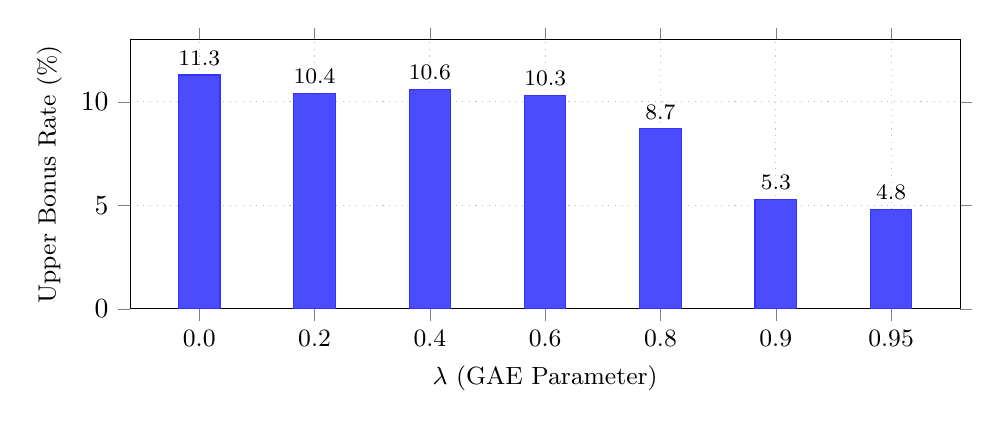
\begin{tikzpicture}
        \begin{axis}[
                ybar,
                width=\columnwidth,
                height=5cm,
                xlabel={$\lambda$ (GAE Parameter)},
                ylabel={Upper Bonus Rate (\%)},
                symbolic x coords={0.0, 0.2, 0.4, 0.6, 0.8, 0.9, 0.95},
                xtick=data,
                xticklabel style={font=\small},
                ylabel style={font=\small},
                xlabel style={font=\small},
                bar width=15pt,
                ymin=0, ymax=13,
                grid=both,
                grid style={dotted},
                tick align=outside,
                nodes near coords,
                nodes near coords style={font=\footnotesize, anchor=south},
            ]

            \addplot[
                fill=blue!70!white,
                draw=blue!80!white,
                error bars/.cd,
                y dir=both,
                y explicit
            ] coordinates {
                    (0.0, 11.3)
                    (0.2, 10.4)
                    (0.4, 10.6)
                    (0.6, 10.3)
                    (0.8, 8.7)
                    (0.9, 5.3)
                    (0.95, 4.8)
                };

        \end{axis}
    \end{tikzpicture}
    \caption{Upper bonus achievement by GAE lambda}
    \label{fig:gae-lambda-bonus}
\end{figure}
